% ===================================================================
%  Week 2 — Point Operations & Histograms
%  Compile: pdflatex -interaction=nonstopmode slides.tex  (twice)
% ===================================================================
\documentclass[10pt,aspectratio=169]{beamer}
% ===================================================================
%  Shared Beamer preamble for "Practical Image Processing"
%  English slides. Compile with pdfLaTeX.
% ===================================================================

\usetheme{metropolis}
\usepackage[T1]{fontenc}
\usepackage[utf8]{inputenc}
\usepackage{lmodern}
\usepackage{listings}
\usepackage{tcolorbox}
\usepackage{fontawesome5}
\usepackage{booktabs}
\usepackage{amsmath,amssymb}
\usepackage{tikz}
\usepackage{pgfplots}
\pgfplotsset{compat=1.17}
\usetikzlibrary{arrows.meta,positioning,shapes.geometric,fit,backgrounds,matrix}
\tcbuselibrary{skins,breakable}

% ---- Palette --------------------------------------------------------
\definecolor{coursePrimary}{HTML}{1B4965}   % deep blue
\definecolor{courseAccent}{HTML}{E76F51}    % coral
\definecolor{courseGood}{HTML}{2A9D8F}      % teal
\definecolor{courseBad}{HTML}{C0392B}       % red
\definecolor{courseInfo}{HTML}{2980B9}      % blue
\definecolor{codeBg}{HTML}{F5F6FA}
\definecolor{codeKw}{HTML}{8E44AD}
\definecolor{codeStr}{HTML}{2A9D8F}
\definecolor{codeCom}{HTML}{7F8C8D}

\setbeamercolor{frametitle}{bg=coursePrimary}
\setbeamercolor{progress bar}{fg=courseAccent}
\setbeamercolor{alerted text}{fg=courseAccent}
\metroset{block=fill,sectionpage=progressbar,numbering=fraction}

% ---- Code listings (Python is built into listings) -----------------
\lstdefinestyle{course}{
  backgroundcolor=\color{codeBg},
  basicstyle=\ttfamily\scriptsize,
  keywordstyle=\color{codeKw}\bfseries,
  stringstyle=\color{codeStr},
  commentstyle=\color{codeCom}\itshape,
  numberstyle=\tiny\color{codeCom},
  numbers=left, numbersep=6pt,
  showstringspaces=false, breaklines=true, breakatwhitespace=true,
  tabsize=4, columns=fullflexible,
  frame=single, framesep=4pt, rulecolor=\color{gray!30},
  keepspaces=true, upquote=true, language=Python,
}
\lstset{style=course}
\lstdefinelanguage{bash}{
  keywords={cd,pip,python,venv,source,import}, sensitive=true,
  morecomment=[l]{\#}, morestring=[b]', morestring=[b]",
}

% ---- Reusable callout boxes ----------------------------------------
\newtcolorbox{goodbox}[1][Good practice]{colback=courseGood!8,colframe=courseGood,
  fonttitle=\bfseries,title={\faCheck~#1},boxrule=0.6pt,left=4pt,right=4pt,top=3pt,bottom=3pt}
\newtcolorbox{badbox}[1][Pitfall]{colback=courseBad!8,colframe=courseBad,
  fonttitle=\bfseries,title={\faTimes~#1},boxrule=0.6pt,left=4pt,right=4pt,top=3pt,bottom=3pt}
\newtcolorbox{infobox}[1][Note]{colback=courseInfo!8,colframe=courseInfo,
  fonttitle=\bfseries,title={\faInfoCircle~#1},boxrule=0.6pt,left=4pt,right=4pt,top=3pt,bottom=3pt}
\newtcolorbox{mathbox}[1][Math]{colback=coursePrimary!6,colframe=coursePrimary,
  fonttitle=\bfseries,title={\faCalculator~#1},boxrule=0.6pt,left=4pt,right=4pt,top=3pt,bottom=3pt}

\newcommand{\keyidea}[1]{\begin{alertblock}{Key idea}#1\end{alertblock}}
\newcommand{\term}[1]{\textbf{\color{coursePrimary}#1}}
\newcommand{\code}[1]{\lstinline[basicstyle=\ttfamily\small]|#1|}

% ---- A helper to draw a small pixel grid, cells shaded by value ----
% \pixelgrid{ {10,20,120,200,240}, {30,60,130,180,230}, ... }
\newcommand{\pixelgrid}[1]{%
  \begin{tikzpicture}[font=\scriptsize,scale=0.6]
    \foreach \row [count=\ry] in {#1} {
      \foreach \val [count=\cx] in \row {
        \draw[gray,fill=coursePrimary!8] (\cx,-\ry) rectangle ++(1,-1);
        \node at (\cx+0.5,-\ry-0.5) {\val};
      }
    }
  \end{tikzpicture}}


\title{Point Operations \& Histograms}
\subtitle{Week 2 — Fixing exposure and contrast}
\author{Practical Image Processing}
\date{Lecture 2 \textbullet\ 60--70 min}

\begin{document}

\maketitle

\begin{frame}{Recap \& today}
  \begin{columns}[T]
    \begin{column}{0.58\textwidth}
      \begin{itemize}
        \item Wk1: an image is numbers on a grid; watch BGR, uint8, [y,x].
        \item \alert{Today:} \term{point operations} — transform each pixel by itself — and the
              \term{histogram}, the tool that tells you what a transform should do.
      \end{itemize}
    \end{column}
    \begin{column}{0.42\textwidth}
      \begin{alertblock}{Why it matters}
        DocScan's meter photos are often too dark or low-contrast. Fixing exposure is step one
        to reading the digits.
      \end{alertblock}
    \end{column}
  \end{columns}
\end{frame}

\begin{frame}{Roadmap}\tableofcontents\end{frame}

% ==================================================================
\section{The histogram}
% ==================================================================

\begin{frame}{The histogram: a census of brightness}
  \begin{columns}[T]
    \begin{column}{0.5\textwidth}
      A real meter crop and its histogram:
      \begin{center}
      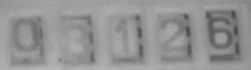
\includegraphics[width=\linewidth]{../assets/gray.png}\\[3pt]
      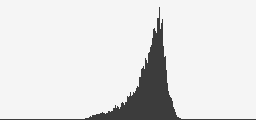
\includegraphics[width=\linewidth]{../assets/hist_before.png}
      \end{center}
    \end{column}
    \begin{column}{0.5\textwidth}
      \begin{itemize}
        \item $x$-axis: intensity 0--255. $y$-axis: how many pixels have it.
        \item This histogram is bunched $\rightarrow$ \term{low contrast} (digits barely stand out).
        \item Read the histogram \emph{before} touching the image.
      \end{itemize}
    \end{column}
  \end{columns}
\end{frame}

\begin{frame}{Reading a histogram}
  \begin{center}
  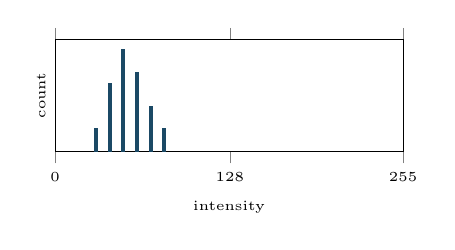
\begin{tikzpicture}
    \begin{axis}[width=6cm,height=3cm,ybar,bar width=1pt,ymin=0,xmin=0,xmax=255,
      xtick={0,128,255},ytick=\empty,font=\tiny,xlabel={intensity},ylabel={count}]
      \addplot[draw=coursePrimary,fill=coursePrimary] coordinates{(30,2)(40,6)(50,9)(60,7)(70,4)(80,2)};
    \end{axis}
  \end{tikzpicture}
  \end{center}
  \begin{itemize}
    \item Peak on the \term{left} = dark (under-exposed). On the \term{right} = bright.
    \item \term{Narrow} = low contrast. \term{Spread across the range} = good contrast.
    \item Two peaks (\term{bimodal}) = object vs background — a gift for thresholding (later today).
  \end{itemize}
\end{frame}

\begin{frame}[fragile]{Computing a histogram}
\begin{lstlisting}[language=Python]
import cv2, numpy as np
gray = cv2.cvtColor(cv2.imread('E:/data/abfa_image/numerators/num_3494.jpg'),
                    cv2.COLOR_BGR2GRAY)
hist = cv2.calcHist([gray], [0], None, [256], [0, 256])  # 256 bins
print(gray.min(), gray.max(), gray.mean())   # quick exposure check
\end{lstlisting}
  \keyidea{The histogram throws away \emph{where} pixels are and keeps \emph{how many} of each value.
  That's exactly what you need to reason about exposure and contrast.}
\end{frame}

% ==================================================================
\section{Point operations}
% ==================================================================

\begin{frame}{Point operations: one pixel at a time}
  \begin{itemize}
    \item A \term{point operation} maps each pixel's value through a function $s = T(r)$ — independent of neighbours.
    \item Brightness: $s = r + b$. Contrast: $s = a\cdot r$. Negative: $s = 255 - r$.
    \item Implemented as a \term{lookup table} (LUT): compute $T$ once for 0--255, apply to all pixels fast.
  \end{itemize}
  \begin{mathbox}
    General linear: $s = a\cdot r + b$ — $a$ scales contrast, $b$ shifts brightness. Then clip to 0--255.
  \end{mathbox}
\end{frame}

\begin{frame}{Gamma correction — on the real meter}
  \begin{columns}[T]
    \begin{column}{0.33\textwidth}\begin{center}
      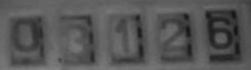
\includegraphics[width=\linewidth]{../assets/gamma_dark.png}\\{\scriptsize $\gamma<1$ (darker)}
    \end{center}\end{column}
    \begin{column}{0.33\textwidth}\begin{center}
      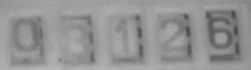
\includegraphics[width=\linewidth]{../assets/gray.png}\\{\scriptsize original}
    \end{center}\end{column}
    \begin{column}{0.33\textwidth}\begin{center}
      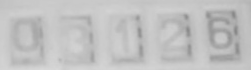
\includegraphics[width=\linewidth]{../assets/gamma_bright.png}\\{\scriptsize $\gamma>1$ (brighter)}
    \end{center}\end{column}
  \end{columns}
  \vspace{4pt}
  \begin{mathbox}
    $s = 255\,(r/255)^{1/\gamma}$ — a \emph{nonlinear} curve that brightens shadows without blowing out highlights.
  \end{mathbox}
\end{frame}

\begin{frame}{Brightness/contrast vs gamma}
  \begin{itemize}
    \item Linear ($a r + b$) shifts/scales everything equally — can clip highlights or crush shadows.
    \item Gamma is \term{nonlinear}: it lifts dark tones more than bright ones (or vice versa).
    \item For a dark meter photo, gamma often recovers digits that a linear brighten would wash out.
  \end{itemize}
  \begin{goodbox}
    Match the tool to the histogram: shifted-but-spread $\rightarrow$ brightness; bunched $\rightarrow$ contrast/gamma.
  \end{goodbox}
\end{frame}

% ==================================================================
\section{Contrast enhancement}
% ==================================================================

\begin{frame}{Contrast stretching (min--max)}
  \begin{columns}[T]
    \begin{column}{0.55\textwidth}
      \begin{center}
      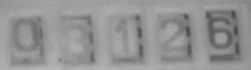
\includegraphics[width=0.9\linewidth]{../assets/gray.png}\\{\scriptsize before}\\[4pt]
      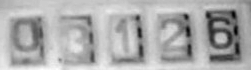
\includegraphics[width=0.9\linewidth]{../assets/stretch.png}\\{\scriptsize after: stretched to 0--255}
      \end{center}
    \end{column}
    \begin{column}{0.45\textwidth}
      \begin{itemize}
        \item Map the actual $[\min,\max]$ to the full $[0,255]$.
        \item Simple, reversible, and it can't invent detail — just uses the full range.
      \end{itemize}
      \begin{mathbox}
        $s = 255\dfrac{r-\min}{\max-\min}$
      \end{mathbox}
    \end{column}
  \end{columns}
\end{frame}

\begin{frame}{Histogram equalization}
  \begin{columns}[T]
    \begin{column}{0.5\textwidth}
      \begin{center}
      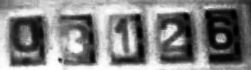
\includegraphics[width=0.85\linewidth]{../assets/equalized.png}\\{\scriptsize equalized meter}\\[3pt]
      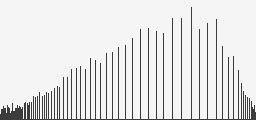
\includegraphics[width=0.85\linewidth]{../assets/hist_after.png}\\{\scriptsize its histogram — spread out}
      \end{center}
    \end{column}
    \begin{column}{0.5\textwidth}
      \begin{itemize}
        \item Redistributes intensities so the histogram is (roughly) \term{uniform}.
        \item Uses the \term{cumulative histogram} (CDF) as the mapping function.
        \item Great for revealing detail in low-contrast images — but can over-amplify noise.
      \end{itemize}
    \end{column}
  \end{columns}
\end{frame}

\begin{frame}[fragile]{The three, in code}
\begin{lstlisting}[language=Python]
stretch = cv2.normalize(gray, None, 0, 255, cv2.NORM_MINMAX)
equalized = cv2.equalizeHist(gray)
lut = np.array([((i/255)**(1/0.5))*255 for i in range(256)], np.uint8)
gamma = cv2.LUT(gray, lut)                 # gamma = 0.5
\end{lstlisting}
  \begin{infobox}
    \code{cv2.LUT} applies a 256-entry table to every pixel in one fast pass — the pattern for any point op.
  \end{infobox}
\end{frame}

% ==================================================================
\section{In-class exercise}
% ==================================================================

\begin{frame}{\faPen~In-class exercise (10 min)}
  \begin{infobox}[Diagnose from the histogram]
  \end{infobox}
  You are handed three meter photos. Their histograms are:
  \begin{enumerate}
    \item a tall spike near 0, nothing above 80;
    \item two separated humps, one near 40 and one near 210;
    \item a smooth spread from 0 to 255.
  \end{enumerate}
  For each: is it under/over-exposed, low-contrast, or fine? Which operation would you apply,
  and which needs \emph{no} enhancement? Which one is easiest to threshold, and why?
\end{frame}

\begin{frame}{\faPen~Debrief}
  \begin{itemize}
    \item (1) Under-exposed \& low-contrast $\rightarrow$ gamma ($\gamma<1$) or stretch; digits hide in the dark.
    \item (2) Bimodal $\rightarrow$ already separable; \emph{ideal} for thresholding (object vs background).
    \item (3) Well-exposed, full range $\rightarrow$ leave it; enhancing may only amplify noise.
  \end{itemize}
  \keyidea{The histogram tells you \emph{whether} and \emph{which} enhancement — before you try anything.}
\end{frame}

% ==================================================================
\section{Thresholding}
% ==================================================================

\begin{frame}{Thresholding: intensity $\rightarrow$ two classes}
  \begin{columns}[T]
    \begin{column}{0.5\textwidth}
      \begin{center}
      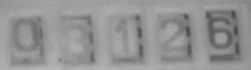
\includegraphics[width=0.9\linewidth]{../assets/gray.png}\\{\scriptsize grayscale meter}\\[4pt]
      
\includegraphics[width=0.9\linewidth]{../assets/otsu.png}\\{\scriptsize Otsu binary: digits vs background}
      \end{center}
    \end{column}
    \begin{column}{0.5\textwidth}
      \begin{itemize}
        \item $s = 255$ if $r>T$ else $0$. Turns gray into black/white.
        \item The whole game is choosing $T$. A bimodal histogram makes it easy.
        \item This is DocScan's ``make it crisp'' step — digits become a clean mask.
      \end{itemize}
    \end{column}
  \end{columns}
\end{frame}

\begin{frame}{Otsu: pick the threshold automatically}
  \begin{itemize}
    \item Otsu's method finds the $T$ that best \term{separates} the two histogram humps.
    \item Formally: minimize the within-class variance (equivalently, maximize between-class variance).
    \item One line: \code{cv2.threshold(g, 0, 255, THRESH\_BINARY+THRESH\_OTSU)}.
  \end{itemize}
  \begin{badbox}
    Otsu assumes two clear classes. On uneven lighting (shadow across the page) a single global $T$ fails — use \emph{adaptive} thresholding.
  \end{badbox}
\end{frame}

\begin{frame}[fragile]{Adaptive thresholding for uneven light}
\begin{lstlisting}[language=Python]
# a local threshold per neighbourhood -> robust to shadows/gradients
binary = cv2.adaptiveThreshold(gray, 255, cv2.ADAPTIVE_THRESH_GAUSSIAN_C,
                               cv2.THRESH_BINARY, blockSize=31, C=10)
\end{lstlisting}
  \keyidea{Global Otsu for even lighting; adaptive for real photos with shadows. DocScan photos usually need adaptive.}
\end{frame}

% ==================================================================
\section{Deep dive}
% ==================================================================

\begin{frame}{CLAHE: local, limited equalization}
  \begin{itemize}
    \item Global equalization over-amplifies noise in flat regions.
    \item \term{CLAHE} equalizes in small tiles and \term{clips} the histogram to limit amplification.
    \item Usually the better default for real photos: \code{cv2.createCLAHE(clipLimit=2.0)}.
  \end{itemize}
  \begin{goodbox}
    For DocScan, CLAHE on the value channel often beats plain equalization — local contrast without the noise blow-up.
  \end{goodbox}
\end{frame}

\begin{frame}{Why equalization can hurt}
  \begin{itemize}
    \item It's data-driven and \term{unpredictable}: two similar images can map very differently.
    \item It amplifies whatever is there — including sensor noise and JPEG blocks.
    \item For a pipeline, prefer a \term{deterministic} op (fixed gamma/stretch) so later stages are stable.
  \end{itemize}
  \keyidea{``Looks better to the eye'' $\ne$ ``better for the next algorithm.'' Enhance for the goal, not the demo.}
\end{frame}

\begin{frame}{Histogram matching}
  \begin{itemize}
    \item Sometimes you want an image's histogram to \emph{match} a reference (consistent look across a dataset).
    \item Useful when meter photos come from many cameras/lightings and you want uniform input.
    \item Map via the two CDFs — the same machinery as equalization, but to a target shape.
  \end{itemize}
\end{frame}

\begin{frame}{Color: enhance value, not each channel}
  \begin{itemize}
    \item Equalizing R, G, B \emph{separately} shifts colors (ugly casts).
    \item Convert to HSV/Lab, enhance the \term{value/lightness} channel, convert back.
    \item Keeps hue intact while fixing brightness/contrast — the correct way to enhance color photos.
  \end{itemize}
  \begin{badbox}
    Per-channel contrast on RGB is a classic beginner mistake that tints the whole image.
  \end{badbox}
\end{frame}

\begin{frame}{Thresholding is a decision, not a default}
  \begin{itemize}
    \item Below $T$ vs above $T$ is a \term{classification} — errors here propagate to every later step.
    \item Too high $T$: digits break up. Too low: background bleeds in. Tune on \emph{hard} images.
    \item Combine: enhance (gamma/CLAHE) $\rightarrow$ then threshold (adaptive) $\rightarrow$ then clean (Week 7 morphology).
  \end{itemize}
\end{frame}

% ==================================================================
\section{Wrap-up}
% ==================================================================

\begin{frame}{What you should now be able to do}
  \begin{itemize}
    \item Read a histogram to diagnose exposure and contrast.
    \item Apply brightness, contrast, gamma, stretching, equalization — and know which fits.
    \item Threshold with a global (Otsu) or adaptive method, and know when each fails.
    \item Enhance color correctly (value channel, not per-RGB).
  \end{itemize}
\end{frame}

\begin{frame}{This week's deliverable}
  \begin{alertblock}{Due before Week 3 (see \code{project/})}
    On real meter/plate images from \code{E:/data}:
    \begin{enumerate}
      \item Plot the histogram; classify each image's exposure/contrast.
      \item Apply and compare: stretch, equalization, gamma, and CLAHE — with before/after.
      \item Produce a clean Otsu \emph{and} adaptive binary of the digits; say which wins and why.
      \item Note: for your DocScan image, which enhancement + threshold combo reads best?
    \end{enumerate}
  \end{alertblock}
\end{frame}

\begin{frame}[standout]
  Look at the histogram first.\\[4pt]
  \normalsize It tells you what the image needs before you change a single pixel.
\end{frame}

\end{document}
